%!TEX root = vmf_main.tex

\section{Format Definition}

VMF is built on top of the JSON format for two principal reasons. Firstly, VMF is composed primarily of ordered collections of integers for time and pitch data along with a header composed of key-value pairs. Because the VMF's representation only requires these two types of data structures, JSON is a perfect fit as JSON arrays provide an ordered collection, and JSON objects provide a collection of key-value pairs. Secondly, because JSON is an extremely popular data format, compatible tools and other parsers are readily available in many different programming languages for consuming the VMF format.

Before describing the format in detail, Figure \ref{fig:completeExample} displays a complete example which can be referenced during the following discussion.

\begin{figure}
  \begin{center}
    \begin{Verbatim}[fontfamily=courier, xleftmargin=\parindent]
    {
      "header": {
        "tick_value": "1",
        "number_of_parts": 2,
        "number_of_voices": 2,
        "time_signature": {
            "0.0": "2/4"
        },
        "key_signature": {
            "0.0": 0
        },
        "tempo": {
          "0.0": 100
        }
      },
      "body": [
        [[1,-1,0,0,4,0],[1,-1,0,0,4,1]],
        [[1,-1,0,4,4,0],[2,-1,0,0,4,1]],

        [[1,-1,0,7,4,0],[1,-1,0,7,4,1]],
        [[1,-1,0,4,4,0],[2,-1,0,7,4,1]]
      ]
    }
    \end{Verbatim}
    \caption{Complete VMF example of a two part score}
    \label{fig:completeExample}
  \end{center}
\end{figure}

\subsection{VMF Header}

In order to interpret the musical data contained in a VMF file, some global information is required for reference. In VMF, this information is stored in the file header. The header object is a JSON object containing information regarding the score's structure, global musical signatures, and the sampling rate produced by the vectors in the body.

The first two header paramters of importance are `'number\_of\_parts`' and `'number\_of\_voices`'. A VMF file is divided into several musical parts which each represent the music played by a single instrument or section. A part is then further subdivided into 1 or more voices. This would cover the case where an instrument is capable of playing more than one melodic line simultaneously such as the guitar or the piano.

The number of parts can be calculated by simply counting the number of individual parts contained in a score. The number of voices in a score is calculated a little bit differently; the maximum number of simultaneous voices in each part must be determined and these maximum values must be added together to arrive at the final value.

For example, when examining Figure \ref{fig:voicesExample}, it is clear that there are four distinct parts (soprano, alto, tenor and bass), and therefore the number of parts recorded in the header would be four. Upon further examination, it can be seen that the soprano, alto and bass parts each have a maximum of 1 voice, while the tenor part has a maximum of 2 voices (measures 1-3). Because of this, the total number of voices in this example is five (the sum of the maximm number of voices in each part).



\begin{figure}
  \begin{center}
    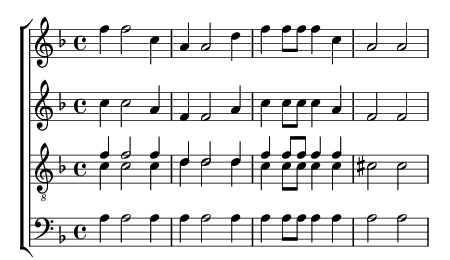
\includegraphics[scale=0.75]{lilypond/voices}
    \caption{Four part, five voice example}
    \label{fig:voicesExample}
  \end{center}
\end{figure}